\chapter{Methodology}

\section{Time Evolutions of Twist-included Brill wave Initial Data}

With the new twist included Brill wave initial data that we constructed, we evolved the initial data in \texttt{BAMPS} NR framework. Unlike the previous tests of Brill waves, we have to evolve the non-diagonal components of the spacetime tensors as well due to the usage of new spatial metric ansatz due to the inclusion of twist. Due to the axisymmetric nature of the problem in hand, we use the cartoon method to simplify the computational costs.

\subsubsection{Cartoon Method \cite{alcubierre_brgmann_holz_takahashi_brandt_seidel_thornburg_2001}}
\label{Cartoon}

In general, performing full 3-D simulations in General Relativity is computationally very expensive due to the dimensionality of the problem. However, when the system possesses axisymmetry, one can exploit this symmetry to significantly reduce computational cost without losing essential physical information.

The cartoon method is a technique that allows one to evolve axisymmetric spacetimes using a reduced computational domain while still employing a Cartesian grid. Instead of evolving the full three-dimensional domain, the evolution is restricted to a thin slab around the symmetry plane (typically the $y=0$ meriodonal plane), consisting of only a few grid points in the symmetry direction.

The key idea is that derivatives in the symmetry direction (e.g., the $y$-direction) can be reconstructed using the assumption of axisymmetry. This is achieved by performing suitable rotations of the evolved variables around the symmetry axis. For a tensor field $T$, its value at off-plane points required for finite difference stencils is obtained by rotating the on-plane data using the Killing symmetry associated with rotations about the axis. Hence essentially our computational domain for the whole problem is the \textbf{Cartesian X-Z} plane.


\subsubsection{Harmonic Damped Wave Gauge (HDWG)}
\label{HDWG}
Harmonic Damped Wave Gauge (HDWG) is obtained by modifying the harmonic gauge condition with a damping term in the gauge source function, turning the coordinate condition into a damped wave equation. This suppresses unphysical gauge modes and stabilizes the coordinate evolution during numerical simulations. The gauge source function for it are

$$
H_a = \mu_L \log \left( \frac{\gamma^p}{\alpha} \right) n_a - \mu_s \alpha^{-1} g_{ai}\beta^i
$$

In black-hole spacetimes, particularly near horizon formation, one often observes a rapid growth of the spatial metric determinant $\gamma$ due to coordinate stretching. The first term in $H_a$, through the logarithmic factor $\log(\gamma^p / \alpha)$, acts to counter this growth by driving a collapse of the lapse $\alpha$, thereby controlling the increase in spatial volume elements. The second term damps the shift vector $\beta^i$, suppressing distortions in the spatial coordinates. For more details, refer \cite{lindblom_szilágyi_2009}

Together, these terms act to control gauge dynamics, preventing the development of large coordinate distortions and stabilizing the evolution near strong-field regions.Since $\mu_L$ and $\mu_s$ sets the time scale where these damping acts, a bit of tuning to find the right parameters are required for proper gauge evolutions which becomes essential in out work.

Using Equation \ref{lapse=shift}, the evolution equation for the lapse and shift becomes, 


\section{Horizon Finding}

In our axisymmetric setting, to locate surfaces satisfying the vanishing expansion condition in Eq.\ref{Horizon}, the problem reduces to a one-dimensional equation in the polar angle, so that the horizon equation becomes an ordinary differential equation. To solve them, we use the \texttt{AHLoc3D} tool which uses a spherical parameterisation for the horizon shape with a parabolic flow method \cite{thornburg_2007}. Essentially, it makes use of guess surfaces in such a way that the outermost MOTS is inside the surface, calculates the expansion at a number of points based on the resolution and the "flows" towards lesser and lesser expansion values based on a pseudo time stepping ($\lambda$), ie
$$
\partial_\lambda x^i = - \Theta s^i
$$
where $s^i$ is the normal vector to the surface.

Additionally in the case of \texttt{AHLoc3D}, the spherical parameterisation used which is $r = F(\theta)$ can only find ray-body/star-shaped horizons. This means that if we draw a ray from the center to the horizon it should only touch horizon once ie the function should not be multivalued in r. This parametrisation begins to break down even before the surface becomes strictly multivalued. In particular, when the surface develops regions where the radial direction becomes tangent to the horizon (i.e., where the outward normal has no radial component), the function $F(\theta)$ develops large gradients or vertical tangents. Numerically, this corresponds to a loss of regularity in the representation, and the horizon finder can fail to converge even though a smooth surface still exists.

Thus, the method is limited not only by true multivaluedness, but also by configurations approaching it, where the surface ceases to be well-described as a function $r(\theta)$.


Despite this limitation, such a parametrisation significantly simplifies the apparent horizon finding problem by reducing it to a one-dimensional equation in $\theta$, making it computationally efficient and straightforward to automate. Consequently, it has become a practical and widely adopted approach in numerical relativity. 
\begin{figure}[!hbt]
    \centering
    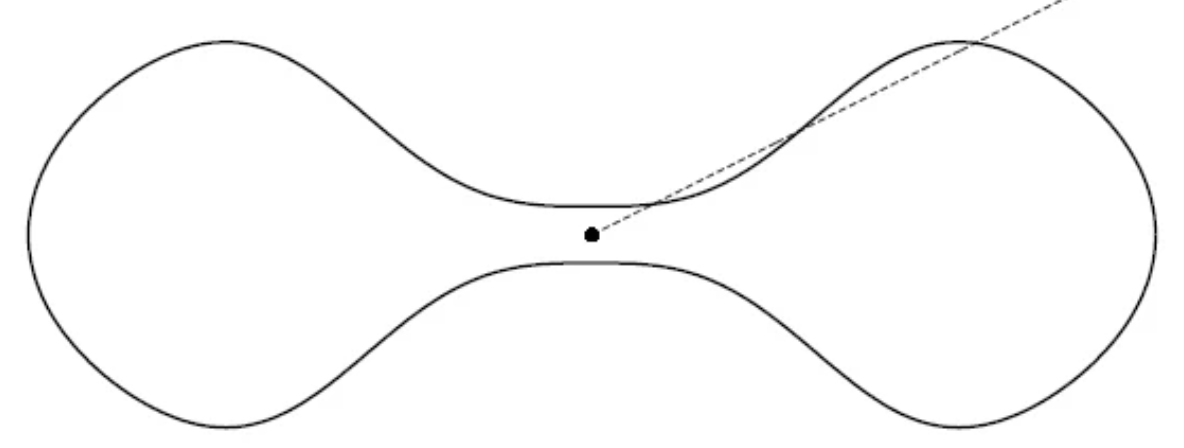
\includegraphics[scale=0.23]{../figures/Screenshot_2026-04-05_14-48-44.png}
    \caption{An example for a non-ray body horizon. Here the r = F($\theta$) parameterisation breaks and \texttt{AHLoc3D} method won't be able find this type of a horizon in the spacetime \cite{thornburg_2007}.}
\end{figure}

Moreover, prior studies of vacuum critical collapse have not indicated the necessity for more general surface representations, as the horizons encountered in those scenarios remain well approximated by star-shaped surfaces. But as we will mention in the coming sections, the inability to tune towards the threshold made us rethink regarding this assumption as a hypothesis which proved to be the correct approach.

We also use a complementary method based on a Cartesian parameterisation with a shooting algorithm, which similarly reduces to solving an ODE in axisymmetry. This removes the ray body limitation that we faced previously but the method uses the Cartoon method as in Sec.\ref{Cartoon} since this search is limited on the y=0 plane and the surface becomes a curve which is parameterised as $X^i (\lambda) = ({X(\lambda),0,Z(\lambda))}$ 

For this method, we integrate the Eq.\ref{Horizon} with this new parameterisation and we get two coupled ODE's of the form in X and Z.

Along the symmetry axis, we begin by making initial guesses for the point at which the horizon intersects the $z$-axis. For each such guess, we integrate the coupled ODEs to obtain a candidate curve $(X(\lambda), Z(\lambda))$. This defines a shooting problem, where we search for solutions that return to the axis, i.e., satisfy $X(\lambda_{\max}) = 0$ for some $\lambda_{\max} > 0$.

In addition to this closure condition, regularity at the axis requires the tangent vector to be aligned with the radial direction in the meridional plane, which imposes the boundary condition $u^z(\lambda_{\max}) = 0$. We therefore select those curves that both return to the axis and satisfy this smoothness condition.

Finally, these candidate solutions are passed to a root-finding algorithm such as \texttt{BRENTQ} to determine the precise initial condition that yields a closed and smooth horizon. For further details, see~\cite{khirnov_2022}.



% Remember to input this to the presentative tex file before compiling.